\end{multicols}
\newpage
\label{bachelor}
\section{Spezielles im Bachelor}
\begin{multicols}{2}

\subsection{Eure Veranstaltungen im ersten Bachelor-Semester}
	Um euch einen kleinen Vorgeschmack auf die Themen zu geben, die euch im ersten Semester beschäftigen werden, gibt es hier einen Überblick:

	\nottoggle{winter}{Je nach euren Vorkenntnissen kann es auch sinnvoll sein, Programmieren 2 oder Technische Informatik 2 zu belegen. Bevor ihr euch dazu entscheidet, solltet ihr euch aber auf jeden Fall durch uns beraten lassen.}{}

\tocheck{0}{Vorlesungsbeschreibungen mit Empfehlungen abgeleichen}

\iftoggle{winter}{
	% !TEX root = ../../../1-te.tex

\subsubsection{Algorithmen und Datenstrukturen}
	\textit{Prof. S\'andor Fekete}
	Diese Vorlesung vermittelt Programmiersprachenunabhängige Algorithmen und Konzepte wie Bäume, Listen oder Stacks. Wer nicht weiß, was sich hinter diesen Begriffen verbirgt, sollte auf keinen Fall die Übungen verpassen.
	% !TEX root = ../../../1-te.tex

\subsubsection{Programmieren 1}
	\textit{Dr. Werner Struckmann}
	In Programmieren 1 geht es um die Programmierung mit Java. Diese Vorlesung eignet sich vorallem für das Home Studium, da sie viele Übungsaufgaben bietet. In Programmieren 2 werden weitere tiefer gehende Programmiertechniken vermittelt. Wer sich schon gut in Java auskennt, kann Programmieren 1 und Programmieren 2 auch im selben Semester machen.
	% !TEX root = ../../../1-te.tex

\subsubsection{Lineare Algebra}
	\textit{Dr. Wolfgang Marten}
	Hier geht es um Vektoren und Matrizen, sowie ein wenig Gruppentheorie. Die Übungen sind zwar nicht immer einfach, geben aber einen sehr guten Ausblick auf die Klausur.
	\subsubsection{Diskrete Mathematik}
	\textit{Prof. Arnfried Kemnitz und PD JP Bode}
	Diskrete Mathematik handelt von allem, was mit ganzen Zahlen zu tun hat: Fibbonacci-Zahlen, Primzahlen, Modulorechnung, usw. Es werden die wichtigsten Mathemaischen Grundlagen vermittelt, unter anderem in Logik, Kombinatorik, Zahlentheorie und Algebra. Die kleinen Übungen sind hier eine sehr gute Vorbereitung auf die Hausaufgaben und die Klausur.
	\subsubsection{Theoretische Informatik 1}
	\textit{Dr. Jürgen Koslowski}
	Hier geht es um formale Sprachen und Automatentheorie. Klingt theoretisch und mathelastig? Ist es auch. Nicht gleich aufgeben, wenn man in der Vorlesung nicht mitkommt, die kleinen Übungen helfen beim Verständnis und bei der Klausurvorbereitung. Sie ist regulär für das dritte Semester vorgesehen, wer es sich zutraut kann sie aber schon im ersten hören und sich damit den Stundenplan im dritten Semester ein wenig freihalten. 
	\subsubsection{Mathewahlpflicht}
%	\textit{N.N.} 
Ihr müsst insgesamt zwei Module zu je fünf Credits
	im Mathe-Wahlpflichtbereich einbringen. Dabei wird eine Vorlesung im Wintersemester und zwei
	Vorlesungen im Sommersemester	angeboten:
	\begin{itemize}
	  \item Sommersemester: 
	    \begin{itemize} 
	      \item Algebra für Informatiker: Hier gehts um grundlegende
		algebraische Strukturen (Mengen, Gruppen, Monide etc). Diese sind insbesondere für die
		theoretische Informatik von großer Bedeutung.
	      \item Einführung in die Stochastik für Informatiker: Die
		Vorlesung behandelt die Grundlagen der
		Wahrscheinlichkeitstheorie (Laplace- Experimente,
		Erwartungswerte, Zufallsvariablen etc.). 
	    \end{itemize}
	  \item Wintersemester: 
	    \begin{itemize}
	      \item Einführung in die Numerik für Informatiker: Hier
		werden Verfahren zum Lösen numerischer Probleme
		behandelt. 
%	      \item Statistische Verfahren für Informatiker: Hier geht
%		es um statistische Probleme und wie man sie lösen kann.
%		Achtung: Die Vorlesung baut auf  ,,Einführung in
%		die Stochastik'' auf und setzt deren Inhalte voraus! Sie wird jedoch derzeit nicht angeboten.
	    \end{itemize}
	\end{itemize}
	Bei der Auswahl geht ihr am Besten so vor, dass ihr euch erstmal
	in alle gerade angebotenen reinsetzt und dann die behaltet, mit der ihr besser
	klarkommt. Generell gilt aber bei mathematischen Vorlesungen: Es
	gibt im Allgemeinen kein aktuelles Skript, wer nichts verpassen
	will, muss in der Vorlesung mitschreiben. Auch können die
	Hausaufgaben gerne mal umfangreicher werden, bereiten aber dafür
	sehr gut auf die Klausur vor. Dranbleiben und sich nicht
	entmutigen lassen ist alles :)
}{
	% !TEX root = ../../../1-te.tex

\subsubsection{Einführung in die Logik}
	\textit{Prof. Koslowski}
	Die Vorlesung behandelt die Grundlagen der formalen Logik, mit einen starken Fokus auf Aussagen- und Prädikatenlogik. Die Hausaufgaben sind dabei teilweise sehr zeitaufwändig, aber dafür eine gute Klausurvorbereitung. Dabei ist das Skript sehr hilfreich.
	% !TEX root = ../../../1-te.tex

\subsubsection{Analysis}
	\textit{Dr. Wolfgang Marten}
	Hier geht es um Differential- und Integralrechnung, sowie Grenzwerte. Die Übungen sind zwar nicht immer einfach, geben aber einen sehr guten Ausblick auf die Klausur. Die Übungsaufgaben sollte man umbedingt machen, wenn man vorhat die Klausur zu bestehen.
	\subsubsection{Computernetze 1}
	\textit{Prof. Lars Wolf}
	Hier lernt man die grundlegende Funktionsweise von Netzwerken kennen. Für die Klausur sollte man auf gar keinen Fall die Übungen verpassen. Interessiert man sich über die Vorlesung hinaus für das Thema, sollte man in die Bücher von Andrew S. Tanenbaum schauen.
	\subsubsection{Mathewahlpflicht}
%	\textit{N.N.} 
Ihr müsst insgesamt zwei Module zu je fünf Credits
	im Mathe-Wahlpflichtbereich einbringen. Dabei wird eine Vorlesung im Wintersemester und zwei
	Vorlesungen im Sommersemester	angeboten:
	\begin{itemize}
	  \item Sommersemester: 
	    \begin{itemize} 
	      \item Algebra für Informatiker: Hier gehts um grundlegende
		algebraische Strukturen (Mengen, Gruppen, Monide etc). Diese sind insbesondere für die
		theoretische Informatik von großer Bedeutung.
	      \item Einführung in die Stochastik für Informatiker: Die
		Vorlesung behandelt die Grundlagen der
		Wahrscheinlichkeitstheorie (Laplace- Experimente,
		Erwartungswerte, Zufallsvariablen etc.). 
	    \end{itemize}
	  \item Wintersemester: 
	    \begin{itemize}
	      \item Einführung in die Numerik für Informatiker: Hier
		werden Verfahren zum Lösen numerischer Probleme
		behandelt. 
%	      \item Statistische Verfahren für Informatiker: Hier geht
%		es um statistische Probleme und wie man sie lösen kann.
%		Achtung: Die Vorlesung baut auf  ,,Einführung in
%		die Stochastik'' auf und setzt deren Inhalte voraus! Sie wird jedoch derzeit nicht angeboten.
	    \end{itemize}
	\end{itemize}
	Bei der Auswahl geht ihr am Besten so vor, dass ihr euch erstmal
	in alle gerade angebotenen reinsetzt und dann die behaltet, mit der ihr besser
	klarkommt. Generell gilt aber bei mathematischen Vorlesungen: Es
	gibt im Allgemeinen kein aktuelles Skript, wer nichts verpassen
	will, muss in der Vorlesung mitschreiben. Auch können die
	Hausaufgaben gerne mal umfangreicher werden, bereiten aber dafür
	sehr gut auf die Klausur vor. Dranbleiben und sich nicht
	entmutigen lassen ist alles :)
	% !TEX root = ../../../1-te.tex

\subsubsection{Programmieren 2}
	\textit{Dr. Werner Struckmann}
	In Programmieren 1 (jährlich im Wintersemester) geht es um
	grundlegende Konzepte der Programmierung am Beispiel von Java.
	Darauf aufbauend wird in Programmieren 2 (jährlich im
	Sommersemester) die Implementierung von Algorithmen und
	Datenstrukturen geübt. Hat man schon gute Vorkenntnisse in einer
	Programmiersprache (etwa durch eine Ausbildung zum
	Fachinformatiker o.Ä.) kann man sich durchaus auch schon im 1.
	Semester an Programmieren 2 versuchen, die Reihenfolge ist NICHT
	vorgeschrieben. 
	% !TEX root = ../../../1-te.tex

\subsubsection{Technische Informatik 2}
	\textit{Prof. Rolf Ernst}
	Das Modul besteht aus Technischer Informatik 1 und 2 und endet
	mit einer Kombiklausur aus beiden Veranstatungen, die
	Reihenfolge in der man diese besucht ist egal, da die
	Inhalte relativ unabhängig voneinander sind.
	Die Vorlesung zu Technischen Informatik 2 orientiert sich
	weitgehend an dem Lehrbuch \enquote{Logic and Computer Design
	Fundamentals – 4th edition} von M. Mano und Ch. Kime, welches
	gleichzeitig als Skript gilt. Das Buch findet man in
	ausreichender Anzahl in der UB. Die kleinen Übungen sind als
	Klausurvorbereitung zu empfehlen, ersetzen aber nicht das eigene
	Nacharbeiten. Wichtig: Belegt man Technische Informatik 2 schon
	im 1. Semester, ist dies nur sinnvoll, wenn man auch Technische
	Informatik 1 im 2. Semester hört, um die Kombiklausur
	mitzuschreiben. Man sollte sich also gut überlegen, wie weit man
	sich da schon festlegen möchte! Andererseits hat man dann im
	zweiten Semester schon ein relativ dickes Modul abgeschlossen,
	was ja auch nicht verkehrt ist.
}

% !TEX root = ../../1-te.tex

\subsection{Interview mit PD Dr. Bode}
	Privatdozent Dr. Bode leitet die große Übung zur Vorlesung \emph{Diskrete Mathematik für Informatiker}, die jährlich im Wintersemester stattfindet. Er hat sich freundlicherweise für ein Interview zur Verfügung gestellt.
	\begin{description}
		\item[Was und wo haben Sie studiert?] 

		Ich habe hier an der Technischen Universität Mathematik mit Nebenfach Informatik studiert. Neben dem Diplom in Mathe habe ich dazu noch das Vordiplom in Informatik gemacht.
		\item[Welchen Bezug haben Sie als Mathematiker zu Informatik?] 

		Für mich sind Computer in erster Linie ein Werkzeug, um bestimmte mathematische Probleme zu lösen. Im Studium habe ich dazu hauptsächlich Vorlesungen aus der theoretischen Informatik gehört. Daneben habe ich als studentische Hilfskraft die Vorlesungen\emph{Theoretische Informatik 1/2} betreut.
		\item[Worum geht es in der Veranstaltung \emph{Diskrete Mathematik für Informatiker}?] 

		Sie behandelt wichtige Grundlagen, die die Studierenden später brauchen werden. Inhaltlich geht es zunächst um allgemeine Grundlagen, bevor wir uns etwas Kombinatorik, Zahlentheorie und Algebra angucken.
		\item[Welche Rolle spielen dabei die Übungen?] 

		Nun, die Übungen sind eine Ergänzung zur Vorlesung, die beim Verständnis helfen sollen. Dazu sind sie eine gute Vorbereitung für die Klausur. Dies klappt aber nur bei aktiver Mitarbeit der Studierenden. Man sollte sich die Aufgaben schon vorher mal angeguckt haben, sonst bringt das nichts.\footnote{Anmerkung des Interviewers: Das kann ich aus eigener Erfahrung bestätigen, auch wenn man dabei noch nichts versteht :)} Die Meisten verhalten sich leider am Anfang sehr passiv.
		\item[Was können Sie den Studierenden für die ersten Semester mit auf den Weg geben?] 

		Sie sollten  nicht alles glauben, was man ihnen erzählt. Vorletztes Jahr gab es das Gerücht, dass unsere 1. große Übung ausfällt, da es ja noch keine Vorlesung gab. Dem war nicht so, wir haben da die Übungseinteilung gemacht. Da weniger anwesend waren, gab es am Ende nicht so viele Übungen, wie man eigentlich gebraucht hätte. Im Zweifelsfall gilt die Webseite zur Übung \verUrl{0}{http://www.mathematik.tu-bs.de/jpbode/dm/}. Dort werden auch die Übungsblätter veröffentlich.\\ Neben diesen speziellen Ratschlag noch einen Allgemeinen: Niemand wird dafür umgebracht, Fragen zu stellen. Wenn also etwas unklar ist, nur Mut!
		\item[Vielen Dank für das Interview!] 

		Bitte sehr. Zum Abschluss möchte ich allen Erstsemestern noch viel Spaß und Erfolg im Studium wünschen.
	\end{description}
	%comic


%muss im master, aber wo passt das rein?
%
\subsection{Stunden- und Semesterplan}
 
Im Vergleich zum Bachelorstudium an der TU-BS bietet der Master
verblüffende Freiheiten in der Fächerwahl. Auch wer die Redewendung
bisher dumm fand, lernt spätestens hier was "`die Qual der Wahl"'
bedeutet. Daher sind dieses und die folgenden Unterkapitel auch in erster
Linie für Masterstudenten gedacht. Allerdings werden mit einigen
Themen auch Bachelorstudenten in Berührung kommen, aber erst ab den
3. Semester. Bei Unterschieden zwischen den Studiengängen gehen wir
kurz darauf ein.\\\\
Zu Beginn jedes Semesters muss man sich selbständig entscheiden, welche Fächer man belegen möchte (und kann) und sich danach den Stundenplan zusammenstellen. Im Gegensatz zu den alteingessenen Bacheloranden aus Braunschweig steht man recht unvorbereitet vor einer ganz und gar nicht trivialen Aufgabe, die man am besten noch vor dem ersten Studientag erledigen sollte. Vielleicht hatte dein Bachelor kaum Wahlmöglichkeiten und das Zusammenstellen eines eigenen Stundenplans ist für dich ungewohnt. Und selbst wenn du diese Freiheiten schon im Bachelor hattest, so sind die Rahmenbedinungen und Feinheiten hier sicherlich ganz andere.

Und anders als im Bachelor, bei dem die meisten Vorlesungen erst in der zweiten Woche beginnen, starten viele Mastervorlesungen schon in der ersten Woche, schlimmstenfall schon Montag früh. Die erste Vorlesung zu verpassen ist nun auch nicht so schlimm, aber wenn mans vermeiden kann\ldots Es ist übrigens auch nicht ganz leicht, den Vorlesungsstart eines Faches herauszufinden, somit wirst du in der ersten (und evtl. auch zweiten) Woche oft vor verschlossenen Türen oder leeren Räumen stehen.







\subsection{Studienplan und Reihenfolge}
Mindestens so frei wie die Wahl der Fächer ist auch die Wahl der Reihenfolge, in der man diese belegt. Es kursieren Studienpläne für den Master, die vorschlagen, bestimmte Module im ersten Semester zu machen (z.B. das Seminar), und andere im zweiten und dritten, etc. All dies sind höchstens gut gemeinte Tipps, letzlich muss ja nichtmals die Masterarbeit unbedingt am Ende stehen, und zur Idee, das Seminar im ersten Semester zu belegen, siehe auch den nächsten Absatz\ldots
          




% !TEX root = ../../1-te.tex

\subsection{Studienplan}
	\label{bach_studienplan}
	\tocheck{5}{Stimmt die Anzahl Pflichtveranstaltungen noch? Mit aktuellem Stundenplan abgleichen!}
	Wie du wahrscheinlich bereits in deinem Stundenplan festgestellt hast, musst du im ersten Semester \iftoggle{winter}{vier}{vier} Pflichtveranstaltungen hören. Doch die Bezeichnung Pflichtverantstaltung sagt bloß aus, dass du die Veranstaltung \emph{irgendwann} einmal hören musst, um deinen Bachelor abzuschließen. Die zeitliche Abfolge der Veranstaltungen darfst du aber selbst festlegen. Der Fakultäts-Musterstudienplan bietet hier eine gute Orientierungsmöglichkeit. Du musst dich aber nicht daran halten. Niemand zwingt dich eine Veranstaltung zu hören oder hält dich davon ab. Du kannst dich eigentlich in jede Vorlesung setzen, auch ohne hinterher an der Prüfung teilnehmen zu müssen -- allerdings gibt es dann auch keine Punkte dafür. Hier bieten sich zum Beispiel Module aus dem Wahlplichtbereich Informatik an, die eventuell nur alle 2 Jahre angeboten werden und über mehrere Semester gehen. Bei den (Pflicht-)Modulen der Informatik musst du jedoch beachten, dass einige Module auf anderen aufbauen. Zum Beispiel sollten Programmiergrundlagen in den ersten zwei Semestern erarbeitet werden und mit Theoretische Informatik II wirst du dich schwer tun, wenn du TheoInf I nicht gehört hast.

	Damit sich dein Studium nicht unnötig verlängert, solltest du darauf achten, in jedem Semester rund 30 Leistungspunkte zu erwerben.

\subsection{Quo vadis studens?}

Wie geht das eigentlich, studieren?\\
Wie du lernst, studierst, lebst; ob du brav mitschreibst oder öfter mal ausschläfst kannst und musst du selbst entscheiden. \\
Wann du die vorgeschriebenen Lehrveranstaltungen belegst, liegt ebenfalls in deinem eigenen Ermessen, allerdings: Nachdem, bis auf vier Ausnahmen, klar festgelegt ist was du studieren musst, ergibt sich eine sinnvolle Reihenfolge, da beispielsweise fortgeschrittenes Programmieren ohne Kenntnis von Algorithmen schlicht nicht möglich ist. Nichtsdestotrotz hast du Spielraum, das Studium an deine persönliche Situation anzupassen.
Du wohnst noch zu Hause und brauchst nicht arbeiten? Prima, mach noch Theoretische Informatik I im 1. Semester. Du hast ein Kind und musst nebenbei auch noch arbeiten? Kein Problem, sprich dich mit deinem Mentor ab und mach ein Teilzeitstudium. Die konkreten Vorschriften zum Studium findest du in der Prüfungsordnung.

In kurz: Grundsätzlich musst du Veranstaltungen im Wert von 180 Credit POints (CP) erfolgreich absolvieren, davon 116–121 CP im Bereich Informatik, 35 CP in Mathematik, 14–19 CP für dein Nebenfach und 10 CP für Schlüsselqualifikationen.

Um dir einen sinnvollen Weg durchs Studium zu ermöglichen, gibt es von der Fakultät den Musterstudienplan, der versucht Überschneidungen der Veranstaltungen zu vermeiden. Es gibt aber auch noch einen Alternativstudienplan der Fachgruppe, diesen empfehlen wir dir allerdings nur, wenn du dir den geringen Mehraufwand pro Semester zutraust. Dafür wirst du es sehr genießen, während des SEPs und der Bachelorarbeit nicht so viele Vorlesungen zu haben. 
Ihr seid nicht mehr in der Schule, ihr habt nun Freiheiten, nutzt sie weise und studiert so, wie ihr es für richtig haltet.
%\newpage
\end{multicols}%\newpage
%musterstudien
\begin{minipage}{1.0\linewidth}
%\begin{wrapfigure}{r}{0.5\textwidth}   
\begin{center}     
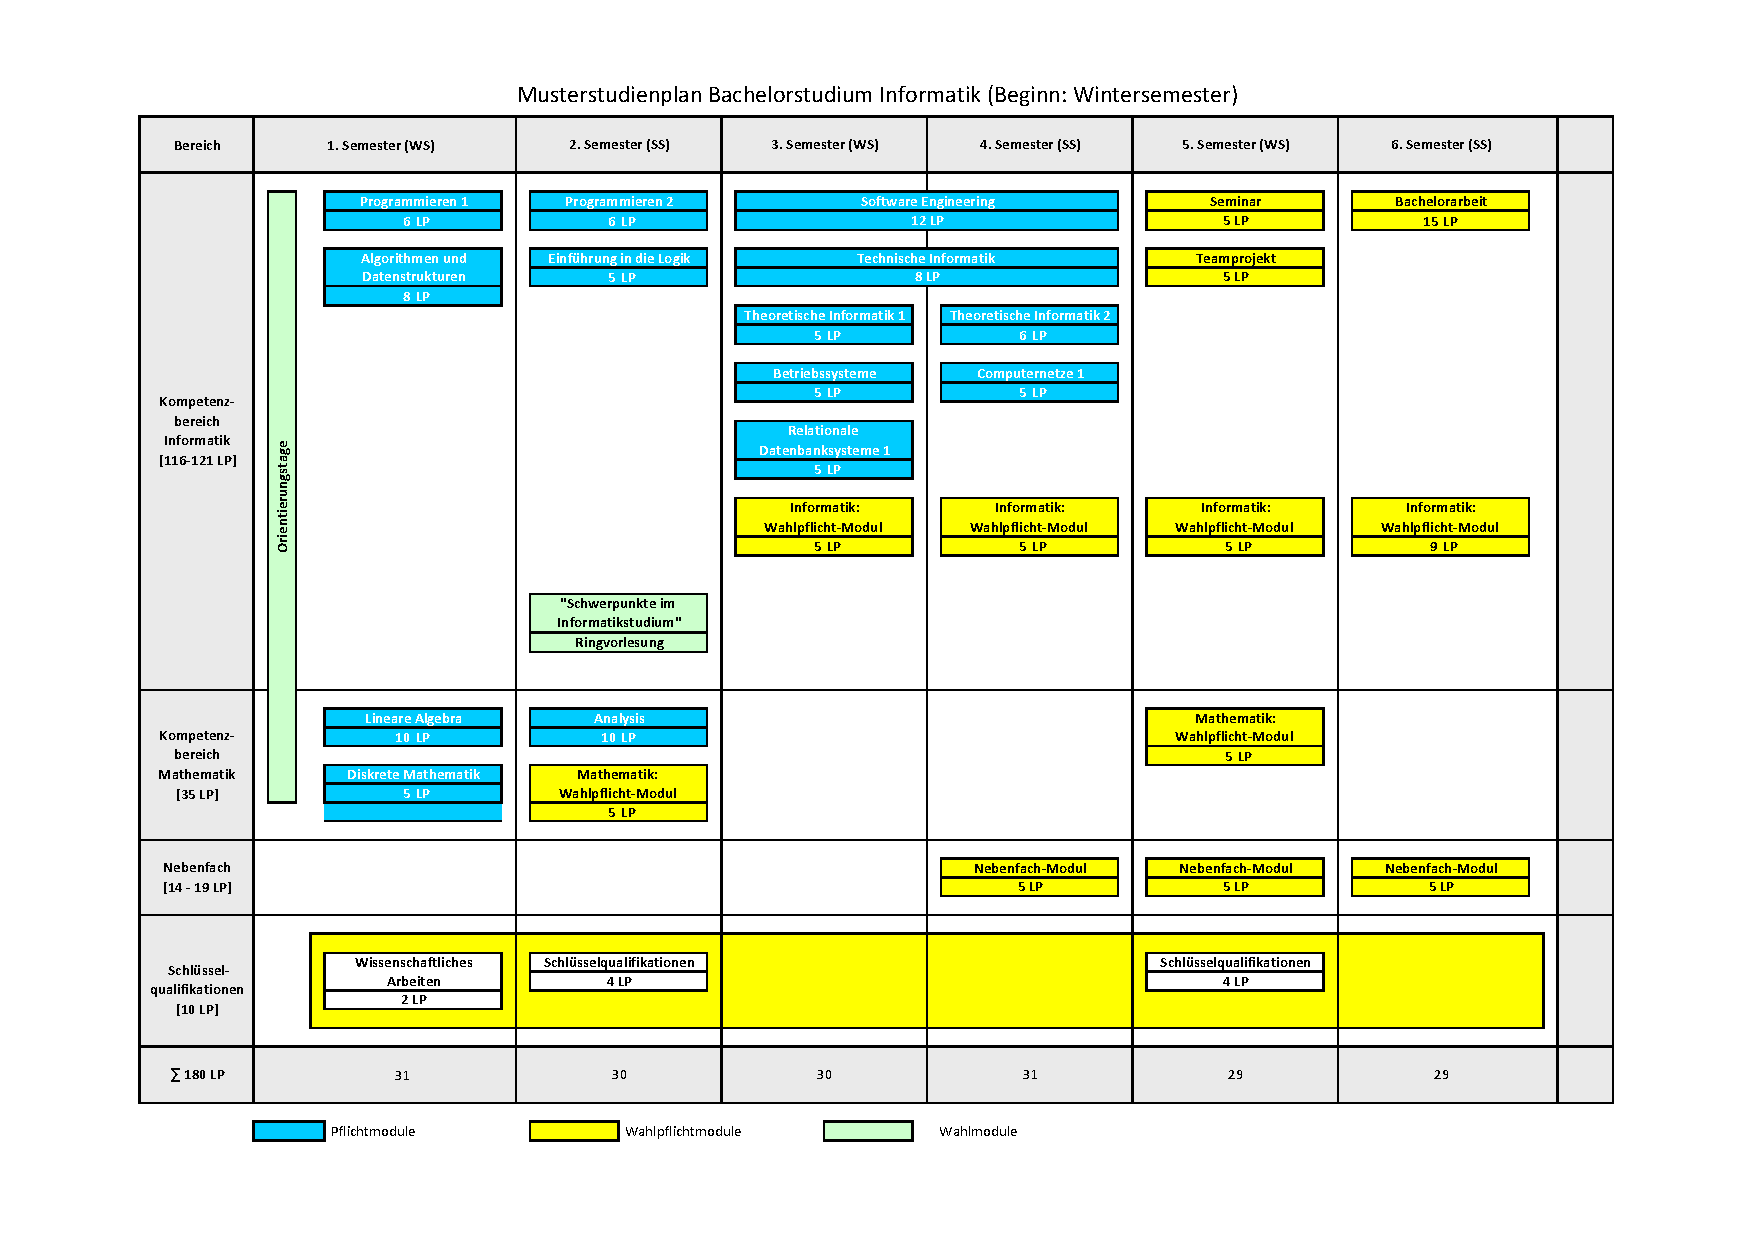
\includegraphics[angle=90,totalheight=\textheight,
  width=\textwidth ]{bilder/Musterstudienplan_BScInformatik_WS_02}
\end{center} 
\label{musterstudienplan}
%\caption{A gull} 
%\end{wrapfigure}
\end{minipage}
\newpage
\begin{minipage}{1.0\linewidth}
%\begin{wrapfigure}{r}{0.5\textwidth}   
%\newpage \
\begin{center}     
%\newpage
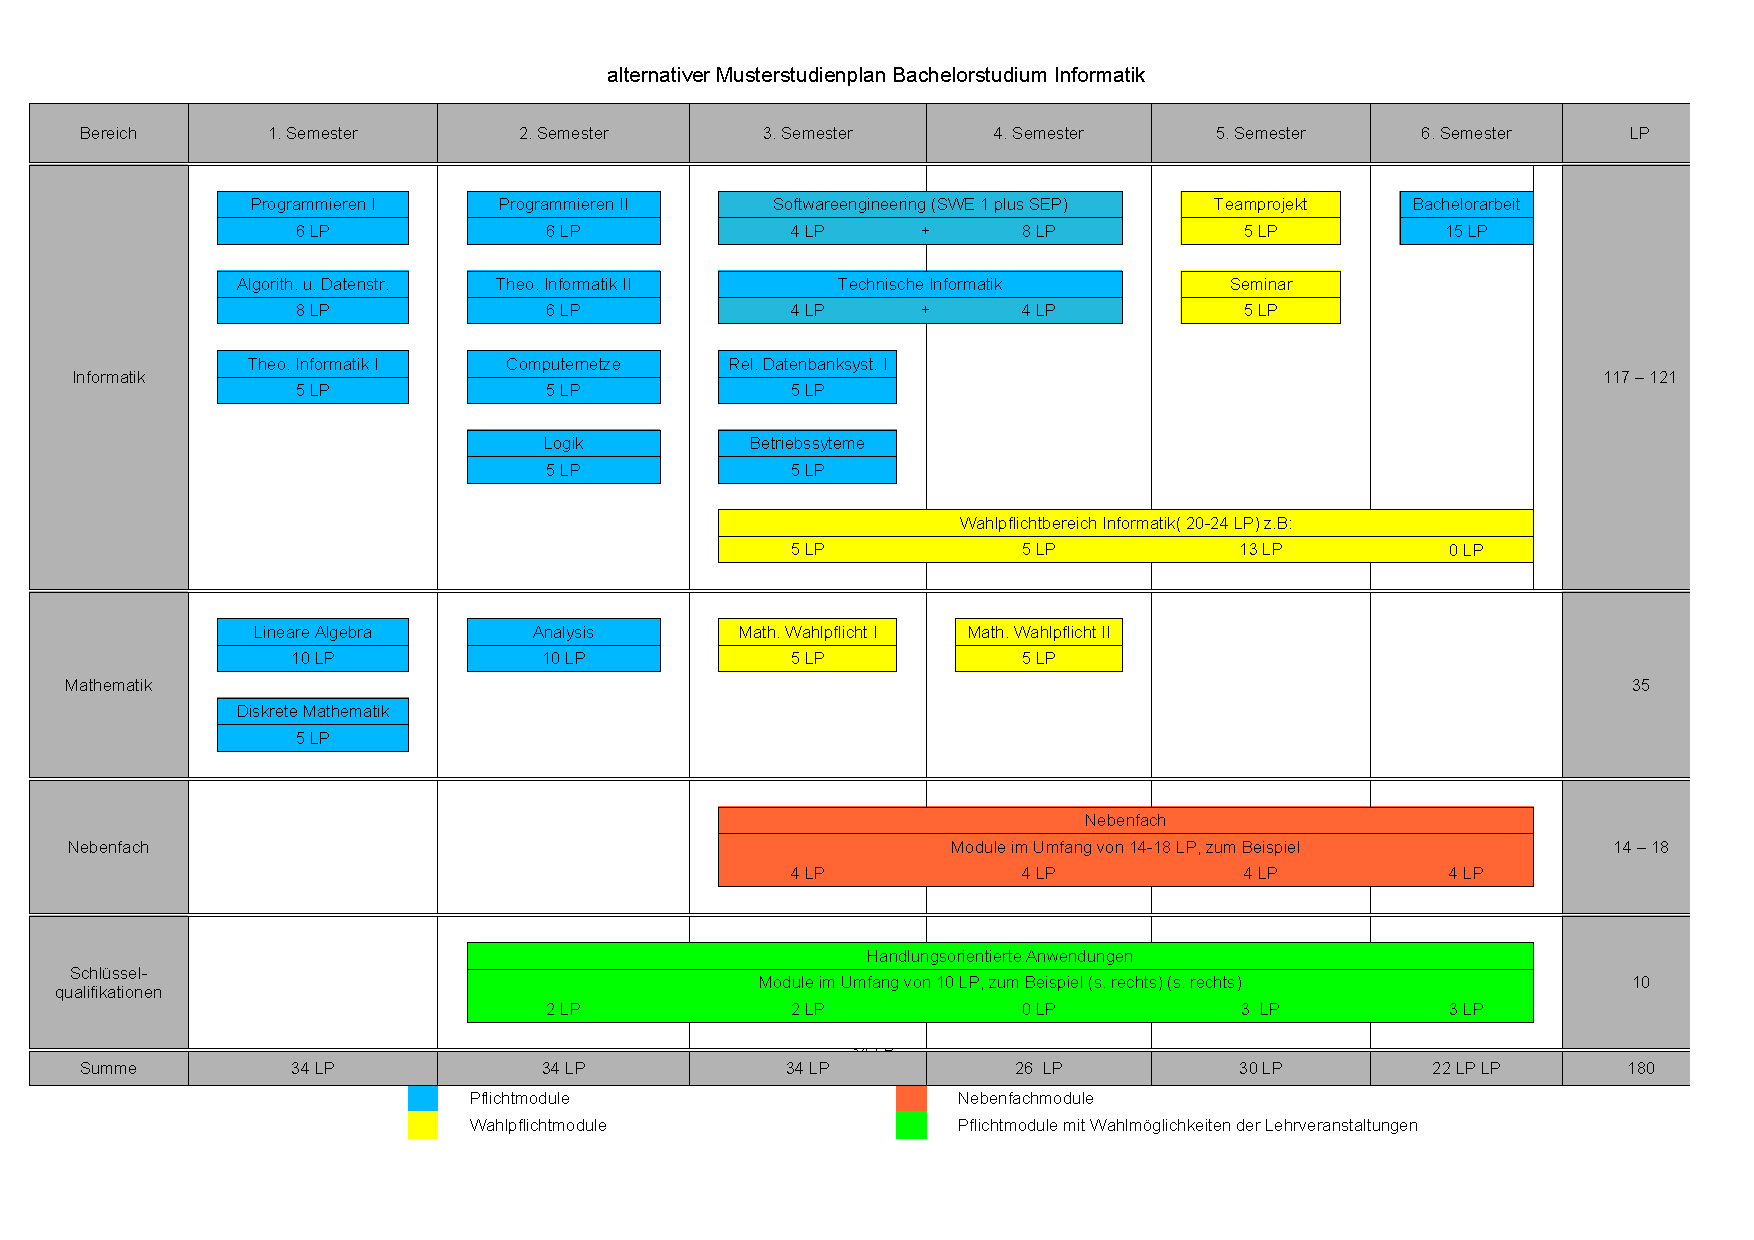
\includegraphics[angle=90,totalheight=\textheight, width=\textwidth ]{texte/bachelor/studienplan_neu.pdf}
\end{center}
%\end{wrapfigure}%\newpage  
\label{studienplan_neu}
\end{minipage} \newpage
%\begin{minipage}
%\newpage
 %Note that we have specified a size for b
%\begin{figure}[h!]
 %% \centering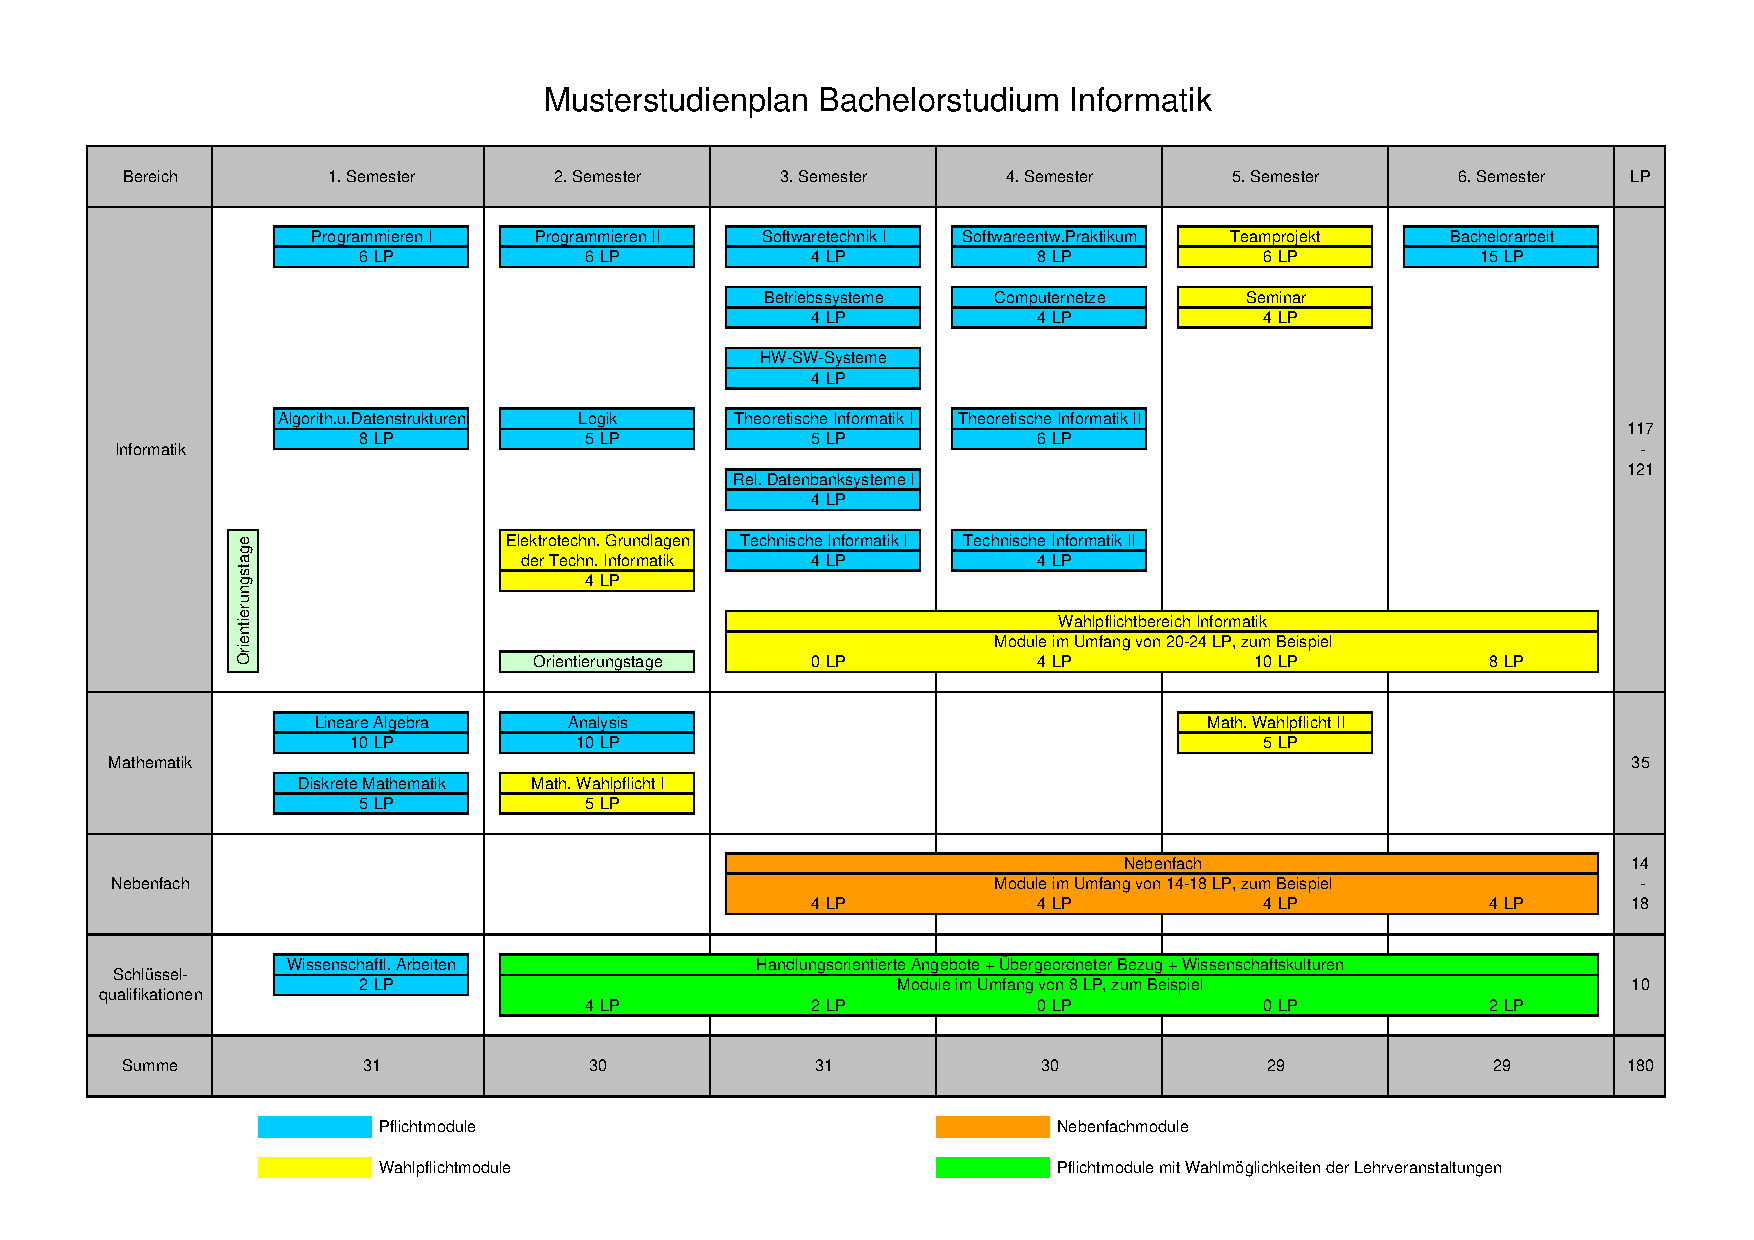
\includegraphics[angle=90,totalheight=\textheight,
%  width=\textwidth ]{texte/bachelor/studienplan.pdf}
%\label{musterstudienplan}
%\end{figure}%\newpage
%\begin{figure}[h!]
  %\centering
\
\ %\newpage \ %\newpage 
\begin{multicols}{2}%\newpage
 %\newpage
\subsection{Studienplanung: Was alles schief gehen kann-
  Leidensbericht eines Fünftsemesters}
\label{studienplan_bericht}
  \textbf{WARNUNG: Dieser Text bezieht sich auf die alte
  Prüfungsordnung und den Studienbeginn im Wintersemester. Somit ist
  für euch nicht alles Weiteres übertragbar.}\\
Nun haben wir euch ja schon eine ganze Menge über die großen
Freiheiten bei der Studienplanung erzählt, sowie sogar noch einen
alternativen Plan vorgelegt. Nun fragt sich sicherlich der Eine oder
Andere, warum es nun noch mehr Text sein muss. Nun, wir dachten uns,
dass Planung gut und schön ist, aber nicht immer klappen muss. Also
dachten wir uns, dass wir am Beispiel eines mäßig begabten Studenten
das mal exemplarisch vorführen, inklusive angepassten
Studienplans. 
Ihr sollt ihr aus seinen Fehlern lernen, was man nicht machen sollte, aber
auch, wie man eigene Fehler noch korrigieren kann. Dazu schreiben wir
jedes Semester, was der Student vorhatte und was es dann geworden ist.
\subsubsection{Prolog}
Als ich anfing, hat uns die Fachgruppe neben der 1-ten uns
insbesondere ihren alternativen Musterstudienplan
\footnote{Die aktuelle Fassung für euch findet ihr auf Seite \pageref{studienplan_neu} - dieser Bericht bezieht sich natürlich 
auf die damalige Fassung für den Start im Wintersemester.}
ans Herz gelegt und
so nahm ich mir denn vor, brav danach zu gehen, aber alles kam ganz
anders...
\subsubsection*{1. Semester}

\newcommand{\nx}{\checkmark}

{
\footnotesize
\begin{tabular}{|l|r|c|c|}
\hline \textbf{Modul}		& \textbf{Credits} 	& \textbf{Plan} & \textbf{Real} \\ 
\hline
\hline Programmieren 1 		& 6 CP 				& \nx 			& \nx 	\\ 
\hline A. u. D.				& 8 CP 				& \nx 			& \nx 	\\ 
\hline Diskrete Mathematik 	& 5 CP 				& \nx 			& \nx 	\\ 
\hline Lineare Algebra 		& 10 CP 			& \nx 			& \nx 	\\ 
\hline Theo. Informatik 1	& 5 CP 				& \nx 			&  		\\ 
\hline Wissens. Arbeiten 	& 2 CP 				& \nx 			& \nx 	\\ 
\hline
\hline Summe 				&  					& 36 CP 		& 31 CP \\ 
\hline 
\end{tabular}
}

%Geplant:
%\begin{itemize}
%\item Programmieren 1 - 6 Credits
%\item Algorithmen und Datenstrukturen - 8 Credits
%\item Diskrete Mathematik - 5 Credits 
%\item Lineare Algebra - 10 Credits
%\item Theoretische Informatik 1 - 5 Credits
%\item Wissenschaftliches Arbeiten - 2 Credits
%\item Summe: 36 Credits
%\end{itemize}
Die Planung ging schon schnell nicht mehr auf, da ich noch damit
überfordet war, alle Hausaufgaben rechtzeitig und selbstständig zu
ersetzen. Insbesondere für Theoretische Informatik 1 war ich zu
unmotiviert und faul, und habe es dann nach den Weihnachtsferien
gekickt. Ich war dabei der Einzige der 5-6 Leute aus meinen Jahrgang,
die der Fachgruppenempfehlung gefolgt waren, alle anderen haben es
erfolgreich durchgezogen. Ich war also erst einmal gefrustet, vor
allem weil es für das Hören eines anderen Faches auch zu spät
war. Somit blieb alles beim offiziellen Musterstudienplan wie auf
Seite \pageref{musterstudienplan}:\\
%Geschafft:
%\begin{itemize}
%\item Programmieren 1 - 6 Credits
%\item Algorithmen und Datenstrukturen - 8 Credits
%\item Diskrete Mathematik - 5 Credits 
%\item Lineare Algebra - 10 Credits
%%\item Theoretische Informatik 1 - 5 Credits
%\item Wissenschaftliches Arbeiten - 2 Credits
%\item Summe: 31 Credits
%\end{itemize}

\subsubsection*{2. Semester}
{
\footnotesize
\begin{tabular}{|l|r|c|c|}
\hline \textbf{Modul}		& \textbf{Credits} 	& \textbf{Plan} & \textbf{Real} \\ 
\hline
\hline Programmieren 2 		& 6 CP 				& \nx 			& 	 	\\ 
\hline Technische Inf. 2	& 4 CP 				& \nx 			& 	 	\\ 
\hline Logik 				& 5 CP 				& \nx 			& \nx 	\\ 
\hline Computernetze 		& 4 CP 				& \nx 			& \nx 	\\ 
\hline Analysis 			& 10 CP 			& \nx 			& \nx	\\ 
\hline Stochastik 			& 5 CP 				& \nx 			& \nx 	\\ 
\hline \LaTeX\ 				& 3 CP 				& \nx 			& \nx 	\\ 
\hline
\hline Summe 				&  					& 37 CP 		& 31 CP \\ 
\hline 
\end{tabular}
}

Da mein Plan mit Theoretische Informatik 2 nicht aufging, musste ich
mir etwas anderes überlegen. Ich war nicht der Einzige und auf der
übrigens sehr empfehlenswerten Seite \url{http://www.clevershit.de/}
fragte jemand nach möglichen Fächern. Wir erfuhren, dass Technische
Informatik 2 trotz des Namens mit etwas Fleiß auch ohne Technische
Informatik 1 als Vorkenntnisse zu schaffen ist. Außerdem wollte ich
nach offiziellen Studienplan ein Mathewahlpflichtfach belegen. Zur
Auswahl standen Stochastik und Algebra. Ich entschied mich für
Stochastik. Dann habe ich  noch kurzfristig eine
Schlüsselqualifikation belegt, und zwar den Kurs ,,Einführung in die
wissenschaftliche Textverarbeitung mit \LaTeX\ '' \footnote{Der
  Anwendung verdankt ihr diesen Text ;)}.%\newpage 
Somit stand die oben gezeigt Planung für das zweite Semester fest.
%das Ergebnis war dann folgende Planung:
%\begin{itemize}
%\item Programmieren 2 - 6 Credits
%\item Technische Informatik 2 - 4 Credits
%\item Logik  - 5 Credits 
%\item Computernetze - 4 Credits
%\item Analysis - 10 Credits
%%\item Theoretische Informatik 1 - 5 Credits
%\item Stochastik - 5 Credits
%\item \LaTeX\ - 3 Credits
%\item Summe: 37 Credits
%\end{itemize}
Allerdings ging auch das nicht auf: Ich hatte in Technische Informatik
2 in der Tat keine Probleme der Vorlesung zu folgen, wenn ich denn mal
da war. Die Hausaufgaben für Stochastik, Programmieren 2, sowie Logik
forderten ihren Tribut und mein Vorlesungsbesuch wurde immer
sporadischer. Entsprechend bin ich dann durch die Prüfung
durchgefallen. Außerdem wollte ich eine gute Note in Analysis, da die
Gewichtung dort sehr stark ist. Entsprechend habe ich mich dann noch
von Programmieren 2 abgemeldet und übrig blieb folgendes:
%\begin{itemize}
%%\item Programmieren 2 - 6 Credits
%%\item Technische Informatik 2 - 4 Credits
%\item Logik  - 5 Credits 
%\item Computernetze - 4 Credits
%\item Analysis - 10 Credits
%%\item Theoretische Informatik 1 - 5 Credits
%\item Stochastik - 5 Credits
%\item \LaTeX\ - 3 Credits
%\item Summe: 27 Credits
%\end{itemize}

\subsubsection*{3. Semester}
{
\footnotesize
\begin{tabular}{|l|r|c|c|}
\hline \textbf{Modul}		& \textbf{Credits} 	& \textbf{Plan} & \textbf{Real} \\ 
\hline
\hline Technische Inf. 1 	& 4 CP 				& \nx 			& 	 	\\ 
\hline Technische Inf. 2 	& 4 CP 				& \nx 			& \nx	\\ 
\hline Relat. Datenb. 1 	& 4 CP 				& \nx 			& 	 	\\ 
\hline HS-Systeme 			& 4 CP 				& \nx 			& \nx	\\ 
\hline Betriebssysteme 		& 4 CP 				& \nx 			& 	 	\\ 
\hline Softwaretechnik 1 	& 4 CP 				& \nx 			& \nx	\\ 
\hline Theoretische Inf. 1 	& 5 CP 				& \nx 			& \nx 	\\ 
\hline Einf. in die Psych. 	& 5 CP 				& \nx 			& 	 	\\ 
\hline Geschichte der Math. & 5 CP 				& \nx 			& \nx	\\ 
\hline SQL-Praktikum		& 4 CP 				& 	 			& \nx 	\\ 
\hline
\hline Summe 				&  					& 39 CP 		& 26 CP \\ 
\hline 
\end{tabular}
}

Im dritten Semester musste ich nun also Theoretische Informatik 1 noch
einmal hören.  Außerdem musste ich ja noch die Klausur in Technische
Informatik 2 schreiben, weil ich diese ja (siehe oben) durch meine
Faulheit versemmelt hatte. Zudem musste ich mit den Nebenfach
anfangen. Ich entschied mich für Psychologie. Im
Schlüsselqualifikationsbereich fehlten mir nur noch 5 Credits. Da mir
eine Mitbewohnerin 
schon von der Vorlesung ,,Geschichte der Mathematik''  erzählt hatte,
und diese genau 5 Credits brachte ergab sich dann die oben gezeigte Planung.
%\begin{itemize}
%%\item Programmieren 2 - 6 Credits
%\item Technische Informatik 1 - 4 Credits
%\item Technische Informatik 2 - 4 Credits
%\item Relationale Datenbanken 1 - 4 Credits 
%\item Hardware-Software-Systeme - 4 Credits
%\item Betriebssysteme - 4 Credits
%\item Softwaretechnik 1 - 4 Credits
%\item Theoretische Informatik 1 - 5 Credits
%%\item Stochastik - 5 Credits
%\item Einführung in die Psychologie - 5 Credits \footnote{Dies ist
%    allerdings geraten, da zum Modul noch zwei andere Prüfungen
%    gehören. Die drei ergeben zusammen 10.}
%\item Geschichte der Mathematik- 5 Credits
%\item Summe: 39 Credits
%\end{itemize}
Natürlich kam es auch hier ganz anders als gedacht: Theoretische
Informatik 1 lief deutlich besser als erwartet, da doch noch
erstaunlich viel vom 1. Semester in Erinnerung geblieben war. Dafür
lief Technische Informatik 1 gar nicht. Spätestens, als unserer
Professor in Relationale Datenbanken, Herr Balke, uns vom
SQL-Praktikum erzählte, dass einen 4 Credits im Wahlpflichtbereich
Informatik einbringt, war mir klar, dass ich dafür Technische
Informatik 1 sausen lassen würde. Aus ähnlichen Gründen scheiterte
Betriebssysteme: Zwei Tage später musste ich Theoretische Informatik 1
schreiben und wieder zwei Tage später Relationale Datenbanken 1. Also
meldete ich mich von Betriebssysteme ab und hoffte so genug Zeit für
die anderen Prüfungen zu haben. Bei Theoretische Informatik 1 klappte
es, bei Datenbanken und Psychologie nicht. Dafür habe ich Technische Informatik 2 im
2. Versuch bestanden und somit blieb es bei 26 Geschafften Punkten.
%\begin{itemize}
%%\item Programmieren 2 - 6 Credits
%%\item Technische Informatik 1 - 4 Credits
%\item Technische Informatik 2 - 4 Credits
%%\item Relationale Datenbanken 1 - 5 Credits 
%\item SQL-Praktikum - 4 Credits
%\item Hardware-Software-Systeme - 4 Credits
%%\item Betriebssysteme - 5 Credits
%\item Softwaretechnik 1 - 4 Credits
%\item Theoretische Informatik 1 - 5 Credits
%\item Geschichte der Mathematik- 5 Credits
%\item Summe: 26 Credits
%\end{itemize}

\subsubsection*{4. Semester}
{
\footnotesize
\begin{tabular}{|l|r|c|c|}
\hline \textbf{Modul}		& \textbf{Credits} 	& \textbf{Plan} & \textbf{Real} \\ 
\hline
\hline Programmieren 2 		& 6 CP 				& \nx 			& \nx 	\\ 
\hline Betriebssysteme 		& 4 CP 				& \nx 			& \nx	\\ 
\hline Relat. Datenb. 1 	& 4 CP 				& \nx 			& \nx 	\\ 
\hline SEP 					& 8 CP 				& \nx 			& \nx	\\ 
\hline Theoretische Inf. 2 	& 6 CP 				& \nx 			&  		\\ 
\hline Chip- \& Systement. 1& 4\footnotemark[\value{footnote}] CP& \nx 		& 	 	\\ 
\hline Netzwerkalgorithmen	& 5 CP 				& \nx 			& \nx \addtocounter{footnote}{1}	\\ 
\hline Mensch im Kontext\footnotemark[\value{footnote}]& 5 CP	& \nx 			& 	 	\\ 
\hline
\hline Summe 				&  					& 42 CP 		& 27 CP \\ 
\hline 
\end{tabular}
}
\addtocounter{footnote}{-1}
\footnotetext[\value{footnote}]{Für den 1. Teil,
    also die Vorlesung plus Prüfung, der 2. Teil folgt im 5. Semester.} 
\addtocounter{footnote}{1}
\footnotetext[\value{footnote}]{Die Vorlesung heißt \textit{Der Mensch im sozialen Kontext/Das Individuum in seiner Entwicklung}. Die Creditzahl ist wieder geraten, da der 2. Teil
 des im 3. Semester angefangenen Moduls, beide ergeben zusammen 10} 
\addtocounter{footnote}{1}

So brach nun das vierte Semester an und somit das
Softwarentwicklungspraktikum (SEP). Nun freute ich mich darüber, schon
Computernetze und Technische Informatik 2 gemacht zu haben, blieb doch
als Pflichtfach nur Theoretische Informatik 2, und dazu noch zwei
Fächer aus der Psychologie, die den Rest des im WS angefangenen Moduls
bilden würden. Dazu kamen noch die Wahlmodule. Ich entschied
mich für Netzwerkalgorithmen, da ich Algorithmen und Datenstrukturen
vom 1. Semester noch in guter Erinnerung hatte. Aufgrund ähnlicher
Erfahrungen mit Hardware-Software-Systeme belegte ich außerdem die
Fortführung ,,Chip- und Systementwurf 1''.  Auch wollte ich endlich
die Klausuren für ,,Betriebssysteme'' und ,,Programmieren 2'', sowie
,,Relationale Datenbanken 1''
nachholen. 
%\begin{itemize}
% \item Programmieren 2 - 6 Credits
% \item Betriebssysteme - 4 Credits
%\item Relationale Datenbanken - 4 Credits
%\item SEP - 8 Credits
%\item Theoretische Informatik 2 - 6 Credits
%\item Chip- und Systementwurf 1 - 4 Credits \footnote{Für den 1. Teil,
%    also die Vorlesung plus Prüfung, der 2. Teil folgt im 5. Semester.}
%\item Netzwerkalgorithmen       - 5 Credits
%%\item Stochastik - 5 Credits
%\item Der Mensch im sozialen Kontext/Das Individuum in seiner Entwicklung - 5 Credits \footnote{Wieder geraten da der 2. Teil
%    des im 3. Semester angefangenen Moduls, beide ergeben zusammen 10}
%%item Geschichte der Mathematik- 5 Credits
%\item Summe: 42  Credits
%\end{itemize}
Mein Plan war also diesmal deutlich reduzierter, da ja ganze 14 Credits
erst zur Prüfungsphase relevant wurden. So dachte ich und so täuschte
ich mich. Das SEP erwies sich in der Tat als so zeitaufwendig und
stressig, wie höhere Semester immer berichtet hatten. Mit Müh und Not
schaffte ich daneben die Zulassung für Netzwerkalgorithmen und
Theoretische Informatik 2. Da ich insbesondere bei letzten Fach nicht
das Gefühl hatte, groß etwas verstanden zu haben, habe ich die Prüfung
dann lieber geschmissen und aufs 6. Semester vertagt. Dafür lief das
SEP und die ,,Altlasten'' unter den Prüfungen deutlich besser: Der
Betreuer war sehr angetan von unserer Arbeit und ich konnte endlich
ein Häkchen hinter Betriebssysteme, Programmieren und Datenbanken
setzen. Auch die mündliche Prüfung in Chip- und Systementwurf 1 lief
sehr gut, allerdings fehlt mir dazu noch das dazugehörige Praktikum. 
Offen bleibt  auch noch das
große Psychologiemodul, da ich ja den 1. Teil erst im Wintersemester
würde wiederholen können.
%\begin{itemize}
%%\item Programmieren 2 - 6 Credits
%%\item Technische Informatik 1 - 4 Credits
%%item Technische Informatik 2 - 4 Credits
%%item Relationale Datenbanken 1 - 5 Credits 
%%item SQL-Praktikum - 5 Credits
%%
%%\item Betriebssysteme - 5 Credits
% \item Programmieren 2 - 6 Credits
% \item Betriebssysteme - 4 Credits
%\item Relationale Datenbanken - 4 Credits
%\item SEP - 8 Credits
%%\item Theoretische Informatik 2 - 6 Credits
%%TODO: Anpassen nach CuSE Prüfung
%%\item Chip- und Systementwurf 1 - 4 Credits \footnote{Für den 1. Teil,
%%    also die Vorlesung plus Prüfung, der 2. Teil folgt im 5. Semester.}
%\item Netzwerkalgorithmen       - 5 Credits
%%\item Stochastik - 5 Credits
%%TODO
%%\item Psycholgoie - 5 Credits \footnote{Wieder geraten da der 2. Teil
%%   des im 3. Semester angefangenen Moduls}
%%item Geschichte der Mathematik- 5 Credits
%\item Summe: 27  Credits
%\end{itemize}

\subsubsection*{5. Semester}
{
\footnotesize
\begin{tabular}{|l|r|c|c|}
\hline \textbf{Modul}		& \textbf{Credits} 	& \textbf{Plan} & \textbf{Real} \\ 
\hline
\hline Seminar 				& 5 CP 				& \nx 			& 	 	\\ 
\hline Teamprojekt	 		& 5 CP 				& \nx 			& 		\\ 
\hline Numerik			 	& 5 CP 				& \nx 			& \nx 	\\ 
\hline Prakt. Chipentwurf	& 6 CP 				& \nx 			& \nx	\\ 
\hline Verhalten \& Prozesse\footnotemark[\value{footnote}]& 6 CP	& \nx 			& \nx	 	\\ 
\hline Einf. in die Psych. 	& 5 CP 				& \nx 			& \nx	\\ 
\hline
\hline Summe 				&  					& 36 CP 		& 22 CP \\ 
\hline 
\end{tabular}
}
\footnotetext[\value{footnote}]{Gesetzmäßigkeiten von Verhalten und mentalen Prozessen} 

%Dazu kommen noch die 4 Credits des ersten Teils vom Chipentwurf
%sowie die 5 Credits aus den Psycholgievorlesungen im 4. Semester,
%also insgesamt 45 Credits.

Fürs fünfte Semester lag nun einiges vor mir: Zum einen das Seminar
und das Teamprojekt. Zum anderen wollte ich nun 
endlich Technische Informatik 1, sowie meine versemmelte Psycholgieklausur nachholen. Außerdem fehlt mir
noch das 2. Mathe-Wahlpflichtmodul (ich entscheide mich für Numerik), sowie  das Praktikum für Chip-
und Systementwurf 1. Im Psychologie fehlt mir dann noch das Modul ,,Gesetzmäßigkeiten von Verhalten und mentalen Prozessen'':
%Außerdem fehlen mir noch 4 Credits im Informatik Wahlpflichtbereich,
%aber es wird ja genug angeboten :)
%\begin{itemize}
%\item Technische Informatik 1 - 4 Credits
%\item Seminar - 5 Credits
%\item Teamprojekt - 5 Credits
%\item Numerik - 5 Credits
%\item Praktikum zum Chipentwurf - 6 Credits
%%\item Wahlpflichtmodul Informatik - 4 Credits
%\item Gesetzmäßigkeiten von Verhalten und mentalen Prozessen - 6
%  Credits
%\item Einführung in die Gebiete der Psychologie - 5 Credits (bereits
%  im 3. Semester gehört, damals aber durchgefallen)
%%\item SEP - 8 Credits
%\item Summe: 36 Credits
%\item Dazu kommen noch die 4 Credits des ersten Teils vom Chipentwurf
% sowie die 5 Credits aus den Psycholgievorlesungen im 4. Semester,
% also insgesamt 45 Credits.
%\end{itemize}
Damit hatte ich mich wieder mal ziemlich verhoben. Ganz gut liefen
dabei noch das Chipentwurfspraktikum, sowie Numerik. Während das
Praktikum einfach Spass machte, war Numerik endlich mal ein einfaches
Mathefach. Auch die Psychologievorlesungen waren mal wieder sehr
interessant, auch wenn ich längst nicht immer da war.  Das Seminar und
das Teamprojekt forderten ihren Tribut, auch wenn beide letzlich nicht
ganz liefen wie gewünscht. Zum Seminarthema fand ich erst keinen
Zugang und am Ende konnte ich das nicht mehr aufholen, weshalb ich es
dann geschmissen habe. Auch das Teamprojekt zog sich ziemlich hin. Wir
hoffen nun, dass wir es in April abschließen werden, also im neuen
Semester. Bei der technischen Informatik rächte sich schließlich meine
Faulheit und es hatte sich mal wieder eine versemmelte Klausur mehr angesammelt.
Von den vorgenommenen 45 Credits habe ich nur einen Bruchteil geschafft.
%\begin{itemize}
%\item Numerik: 5 Credits
%\item Praktikum zum Chipentwurf - 6 Credits
%%\item Wahlpflichtmodul Informatik - 4 Credits
%\item Gesetzmäßigkeiten von Verhalten und mentalen Prozessen - 6
%  Credits
%\item Einführung in die Gebiete der Psychologie - 5 Credits (bereits
%  im 3. Semester gehört, damals aber durchgefallen)
%\item Summe: 22 Credits 
%\end{itemize}
Immerhin war damit mein Nebenfach und Chip- und Systementwurf 1
abgeschlossen, dass ich immerhin insgesamt noch 31 Credits verbuchen
konnte.

\subsubsection*{6. und 7. Semester}
{
\footnotesize
\begin{tabular}{|l|r|c|}
\hline \textbf{Modul}		& \textbf{Credits} 	& \textbf{Plan} \\ 
\hline
\hline Technische Inf. 1 	& 4 CP 				& \nx 			\\ 
\hline Theoretische Inf. 2 	& 6 CP 				& \nx 			\\ 
\hline Seminar				& 5 CP 				& \nx 			\\ 
\hline Teamprojekt 			& 5 CP 				& \nx 			\\ 
\hline 
\hline Bachelorarbeit 		& 15 CP 			& \nx 			\\ 
\hline 
\hline Summe 				&  					& 20 / 15 CP 		\\ 
\hline 
\end{tabular}
}

Auch wenn es schon den Ende entgegen geht, hat sich doch einiges noch
angesammelt, sodass ich die Bachelorarbeit erst im 7. Semester
schreiben werde. Vorher aber muss
ich noch meine letzten Scheine schaffen.
%\begin{itemize}
%\item Sechstes Semester:
%\item
%  \begin{itemize}
%  \item Technische Informatik 1 - 4 Credits
%  \item Theoretische Informatik 2 - 6 Credits
%  \item Seminar: 5 Credits
%  \item Teamprojekt 5 Credits
%  \item Summe: 20 Credits
%  \end{itemize}
%\item Siebtes Semester
%  \begin{itemize}
%  \item Bachelorarbeit: 15 Credits
%  \end{itemize}
%\end{itemize}

% Wenn alles nach Plan klappt, habe ich im 6 Semester also nur noch 21
% Credits zu absolvieren, nämlich 6 für Theoretische Informatik 2, sowie
% 15 Credits für die Bachelorarbeit. 
Da ich in der theoretischen
 Informatik starke Defizite habe, werde ich die Vorlesung wohl nochmal
 hören. Dazu kommt noch das Seminar und der Abschluss des
 Teamprojektes und die Klausur in technischer Informatik 1. Um dort
 nun keine weiteren Verzögerungen zu kriegen, ist die Bachelorarbeit
 also noch in weiter Ferne. Aufmerksamen Lesern wird auffallen, dass
 mir noch Credits fehlen. Dazu muss man wissen, dass ich nach der
 alten Prüfungsordnung studiert habe und einige der Fächer mit 4
 Credits durch einen Prüfungswechsel noch aufgewertet werden, das habe
 ich im Text noch nicht berücksichtigt.\\
Insgesamt hat sich mein Studienplan also
 ganz anders entwickelt als gewünscht.
 % Ihr findet ihn als mahnendes
% Beispiel auf Seite \pageref{studienplan_irre}.
% Meine Erfahrung sagt mir aber, dass wohl auch diese Planung
% wieder nicht ganz hinhauen wird. Andererseits ist man flexibel und es
% ist ja nicht das erste Mal, dass ich Fächer in Studienplan hin und her
% schiebe und somit aus einer blöden Situation noch das beste raus
% hole. Den sich daraus ergebenden Studienplan sieht ihr auf der
% nächsten Seite. 
%  Auch sind meine Angaben beim Nebenfach und den
% Wahlfächern natürlich die, die ich belegt habe und somit natürlich nur
% ein Vorschlag.
\paragraph{Nachbemerkungen}
Diese Geschichte ist mir wirklich so passiert und auch noch nicht
abgeschlossen. %Den derzeitigen sich daraus ergebdenen Studienplan
%findet ihr nun auf der nächsten Seite.
 Die eigentliche Frage ist: Warum steht sie hier? Egotrip des
Autors? Darstellen, wie sch*e alles ist? Zeigen, dass Studenten
manchmal sehr ,,verplante'' Studenten sein können?\\\\
Nun, von allen ein Bisschen, der Hauptsinn ist aber ein Anderer: Diese
kleine Geschichte soll zeigen, dass wirklich nichts fest ist im
Bachelor und man grundsätzlich alles umlegen kann wie man will. Ich
kann meinen Studienplan in der Form übrigens nicht zur Nachahmung
empfehlen, da die Belastung pro Semester stark ungleichmäßig verteilt
ist.  Außerdem gilt für euch eine neue Prüfungsordnung mit anderer
Modulstruktur. Er soll aber zeigen, dass wenn etwas schief geht, man trotzdem
noch etwas retten kann, indem man ein wenig hin und her schiebt. Als
Vorlage eignet er sich trotzdem nicht, da für euch schon ein anderes
Modulhandbuch gilt, und deshalb einige Dinge so wohl nicht mehr
möglich sind (welche standen zum Redaktionsschluß noch nicht
fest). Auch muss ich zugeben, dass der Text nicht ohne Weiteres
verständlich ist. Für
Rückfragen  kann man sich aber gerne bei mir  melden. Die Geschichte ist
auch noch nicht abgeschlossen und dieser Text wird für die nächste
1-te sicherlich noch einmal umgeschrieben. Verbesserungsvorschläge und
weiteres Feedback nehme ich daher  gerne entgegen.\\
\emph{Johannes Starosta -- \nolinkurl{J.Starosta@tu-bs.de}}
%\end{multicols}%\newpage
%\begin{figure}[p]
%  \centering
%\label{studienplan_irre}
%  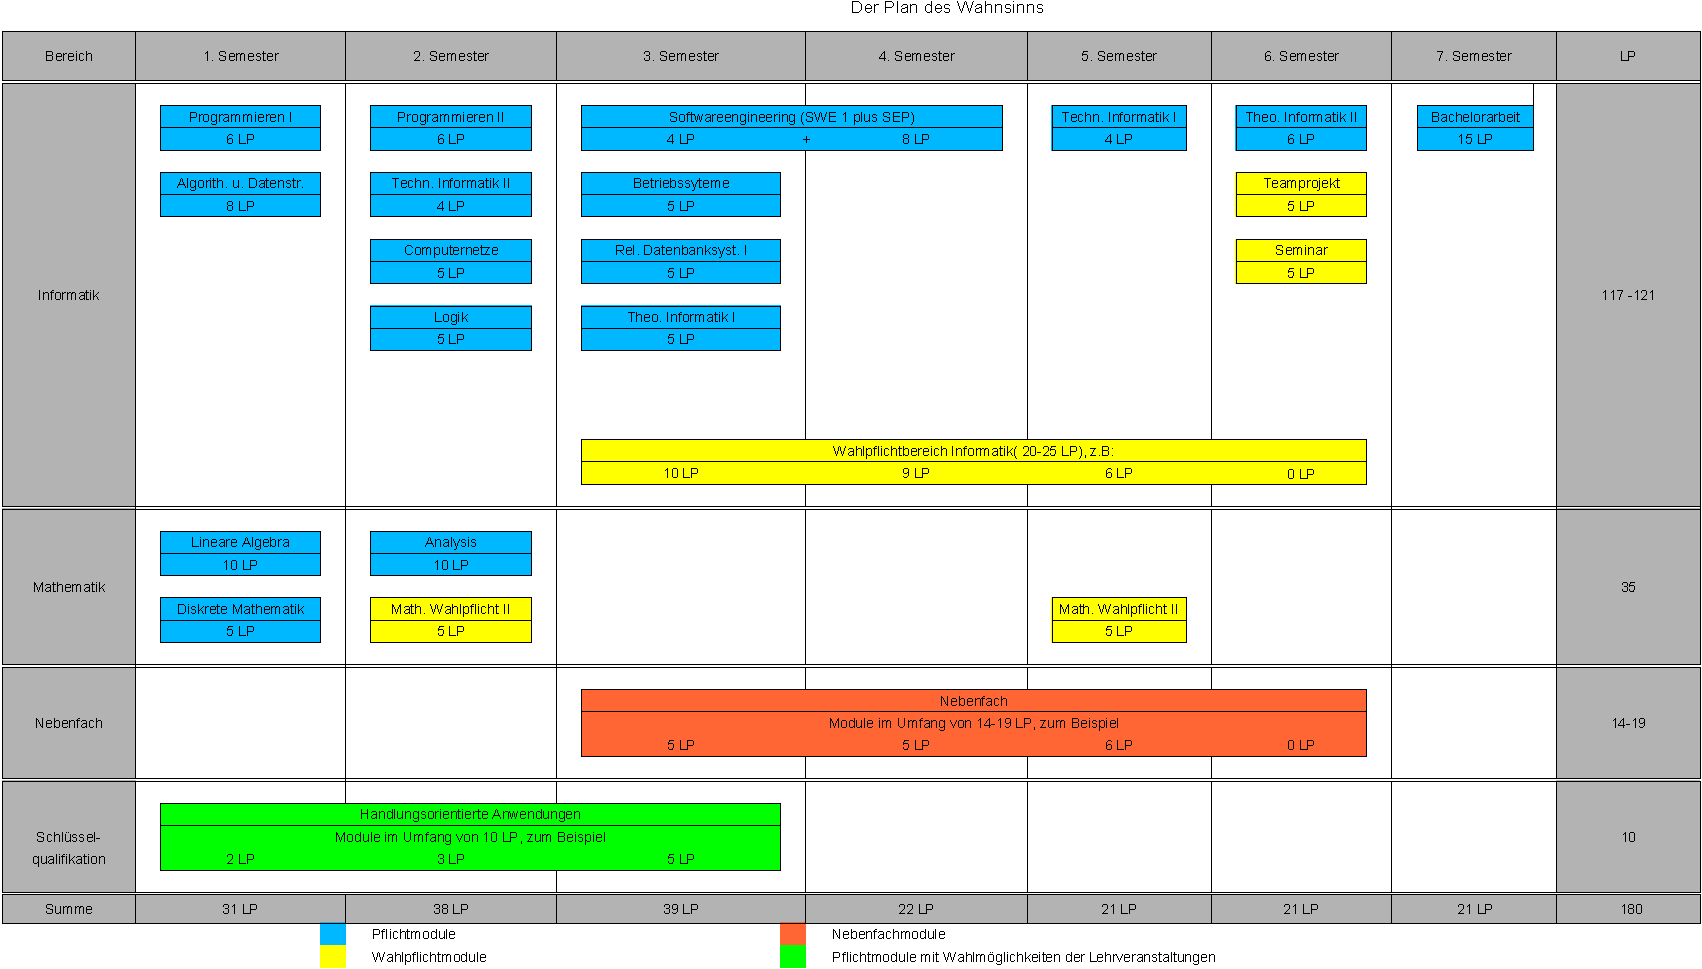
\includegraphics[angle=90,width=0.9\textwidth ]{texte/bachelor/studienplan_joke.pdf}
%\end{figure}
%\begin{multicols}{2}
 % d
%%% Local Variables: 
%%% mode: latex
%%% TeX-master: "../../1-te"
%%% End: 

%%% Local Variables: 
%%% mode: latex
%%% TeX-master: "../../1-te"
%%% End: 
